\chapter{Evaluation}
\label{chap:evaluation}

In this research we have built a specialized inverted index to support users during dataset exploration and SPARQL query building tasks on large-scale RDF datasets. In this chapter we present an evaluation of both the indexing and querying processes described in this work. We will start by posing some questions that our evaluation will address:

\begin{itemize}
    \item How long does the indexing process take?
    \item How much space does indexing require?
    \item How are our times compared against SPARQL endpoint query times?
    \item How do our approximation suggestions compare to precise results?
\end{itemize}

In order to answer these questions, we will first present the experimental settings used for this research.

\section{Experimental setup}

For this work, we have used a personal computer with a i7-4600M CPU @ 2.9GHz and 16GB of RAM, running on Windows 10.

We based our development on the Wikidata dump of March 4\textsuperscript{th} 2018 (20,821,216,963 bytes); and our evaluation of the system with the dump of May 23\textsuperscript{th} 2020 (41,285,029,233 bytes). We had originally developed results from our first Wikidata dump, but we found out that the information in our dataset was outdated, and as consequence, that results against the Wikidata query service were too different to compare.

Regarding the source code, it was written in C\# and tested with \textit{xUnit} with 217 tests and 89\% code coverage. As external packages we have used the following:
\begin{itemize}
    \item For logging, we use \textit{NLog} (v.4.5.10)
    \item \textit{dotnetRDF} (v.2.2.0) is used for RDF handling
    \item For Zip file handling we are using \textit{SharpZipLib} (v.1.0.0)
    \item File types (zip or plain text NTriples) are detected using \textit{Mime} (v.3.0.2)
    \item JSON objects are handled via \textit{Newtonsoft.Json} (v.12.0.2)
    \item Sorting of filtered and inverse triples files is done using \textit{gzip} (v.1.9)
\end{itemize}

% ##############################################################################################
% ##############################################################################################
% ##############################################################################################

\section{Index}

In this section we present metrics for both pre-processing and indexing.

The pre-processing phase gave us the following results:

\begin{table}[h!]
\centering
\begin{tabular}{lrl}
Task                                    & Value  &                    \\
\hline
Size of input file                      & 41,285,029 & KBytes       \\
Number of input triples (lines)         & 5,126,548,635  &            \\
Size of output file                     & 9,184,248 & KBytes        \\
Number of output triples                & 1,098,606,588 &             \\
Runtime duration                        & 34:59:22  & hh:mm:ss        \\
\end{tabular}
\caption{Overview of pre-processing in terms of space and time}
\label{table:preprocessingMetrics}
\end{table}

The indexing process has the following metrics:

\begin{table}[h!]
\centering
\begin{tabular}{lrl}
Task                                    & Value  &                    \\
\hline
Number of input triples                 & 1,098,606,588 &             \\
PageRank runtime duration               & 11:16:25 & hh:mm:ss        \\
Entity index runtime duration           & 58:10:11 & hh:mm:ss       \\
Number of entities                      & 84,623,017 &                \\
Size of entity index                    & 9,721,912 & KBytes         \\
Property index runtime duration         & 5:07:50 & hh:mm:ss       \\
Number of properties                    & 7,559 &                     \\
Size of properties index                & 9,992 & KBytes             \\
Total index size                        & 9,731,904 & KBytes         \\
\end{tabular}
\caption{Overview of indexing in terms of space and time}
\label{table:indexMetrics}
\end{table}

% ##############################################################################################
% ##############################################################################################
% ##############################################################################################

\section{Queries}

We have mentioned before that our system will provide over-approximated suggestions. Readers might wonder how can we measure this? In this section, we would like to show how approximated our results are compared to the exact ones provided from the Wikidata SPARQL endpoint. We will use precision and recall to measure how similar our approximated results are to the exact Wikidata results.

For this, we are going to create a list of sample properties and run queries using these. We expect to get an over-approximation of our suggested values, while not leaving any values outside. In other words, we are expecting that we return all true positives while also having a considerable amount of false positives and low-to-zero false negatives: we expect our over-approximation model to have 100\% recall, with any drop in recall being due to changes in the data between our indexing process, and running the queries on the live SPARQL endpoint.

\subsection{Sample queries}
For our queries, we have created a list of sample properties. Selecting a sample set of properties can be a daunting task: what makes a property a good candidate for testing? A straightforward approach would be to randomly sample properties with equal probability, but most properties in Wikidata have very few triples, while those few properties with more triples are more likely to appear in user queries. Hence the straightforward sampling approach does not seem appropriate. We would rather prefer to have an evaluation set that includes properties with differing numbers of triples (frequency), domain classes and range classes.

We thus decided to create a sample set based on two approaches: random and cherry picking. Since picking properties randomly could return some not-so-interesting properties (low frequency, domain or range), we followed the following approach: First we sorted the properties randomly; we calculated the total sum of the value (e.g.: Sum of all frequencies) that we were looking for and calculated the cumulative contribution to the total. From that total, we took 10 random values between 0-1: this way, we compute a weighted sample where properties are sampled with a probability proportional to their value. This gives us 30 properties: 10 for frequency, domain and range.

For the cherry picking approach, we took an additional 37 properties that had a mix of frequency/domain/range values. We manually selected some properties that had values in between the spectrum of values and added them to the previous list, e.g.: We picked P21 (sex or gender) that has a high frequency, a high domain and a low range. We also picked P301 (category's main topic), that has a high frequency, a low domain and a high range.

We took 67 sample properties in total for our tests. In \autoref{table:sampleProperties1} and \autoref{table:sampleProperties2} we present these. In this table we can observe that there is a mix of high and low values for frequency, domain and range.

\begin{table}[]
\resizebox{\textwidth}{!}{%
\centering
\begin{tabular}{llrrr}
\hline
\multicolumn{1}{l}{\textbf{Prop}} & \multicolumn{1}{l}{\textbf{Label}}  & \multicolumn{1}{l}{\textbf{Freq}} & \multicolumn{1}{l}{\textbf{Domain}} & \multicolumn{1}{l}{\textbf{Range}} \\ 
\hline
P17    & country   & 12418513   & 37642   & 664 \\
P19    & place of birth   & 2460395   & 938   & 3344 \\
P21    & sex or gender   & 6053686   & 2341   & 13 \\
P31    & instance of   & 82929158   & 70082   & 5470 \\
P50    & author   & 8812954   & 2357   & 1019 \\
P102   & member of political party   & 380027   & 116   & 245 \\
P106   & occupation   & 4426526   & 1684   & 1366 \\
P112   & founded by   & 44475   & 3766   & 1378 \\
P127   & owned by   & 386560   & 5262   & 2821 \\
P131   & located in the administrative territorial entity   & 9077756   & 20858   & 3482 \\
P135   & movement   & 49381   & 1358   & 365 \\
P138   & named after   & 252683   & 10147   & 7129 \\
P150   & contains administrative territorial entity   & 76236   & 1155   & 1875 \\
P155   & follows   & 962127   & 8064   & 7955 \\
P156   & followed by   & 955311   & 7837   & 8146 \\
P159   & headquarters location   & 309781   & 5825   & 2390 \\
P180   & depicts   & 151551   & 2134   & 4989 \\
P184   & doctoral advisor   & 24767   & 10   & 16 \\
P276   & location   & 1701029   & 14419   & 4892 \\
P279   & subclass of   & 2427200   & 9631   & 4915 \\
P287   & designed by   & 9745   & 1292   & 242 \\
P301   & category's main topic   & 624932   & 68   & 16273 \\
P361   & part of   & 2137841   & 20309   & 12870 \\
P364   & original language of film or TV show   & 291691   & 552   & 101 \\
P413   & position played on team / speciality   & 337554   & 39   & 62 \\
P421   & located in time zone   & 1491148   & 3004   & 92 \\
P511   & honorific prefix   & 47040   & 61   & 58 \\
P527   & has part   & 551031   & 11313   & 17077 \\
P531   & diplomatic mission sent   & 303   & 4   & 44 \\
P611   & religious order   & 26152   & 319   & 92 \\
P641   & sport   & 1539461   & 7673   & 185 \\
P682   & biological process   & 370975   & 46   & 22 \\
P710   & participant   & 67173   & 1601   & 1639 \\
P793   & significant event   & 107608   & 4342   & 1528 \\
P805   & statement is subject of   & 353   & 201   & 155 \\
P807   & separated from   & 878   & 157   & 171 \\
P873   & phase point   & 23   & 19   & 0 \\
P910   & topic's main category   & 624952   & 16489   & 262 \\
P915   & filming location   & 18844   & 175   & 1334 \\
P921   & main subject   & 7551197   & 3374   & 11388 \\
P971   & category combines topics   & 790631   & 75   & 5702
\end{tabular}}
\caption{Sample properties, part 1}
\label{table:sampleProperties1}
\end{table}

\begin{table}[]
\resizebox{.9\textwidth}{!}{%
\centering
\begin{tabular}{llrrr}
\hline
\multicolumn{1}{l}{\textbf{Prop}} & \multicolumn{1}{l}{\textbf{Label}}  & \multicolumn{1}{l}{\textbf{Freq}} & \multicolumn{1}{l}{\textbf{Domain}} & \multicolumn{1}{l}{\textbf{Range}} \\ 
\hline
P1204   & Wikimedia portal's main topic   & 1654   & 4   & 726 \\
P1344   & participant of   & 240027   & 966   & 1771 \\
P1423   & template's main topic   & 14554   & 21   & 2041 \\
P1424   & topic's main template   & 14095   & 2048   & 46 \\
P1433   & published in   & 35181414   & 1118   & 1008 \\
P1435   & heritage designation   & 1766767   & 7444   & 59 \\
P1445   & fictional universe described in   & 318   & 25   & 197 \\
P1464   & category for people born here   & 34767   & 1295   & 4 \\
P1478   & has immediate cause   & 343   & 156   & 155 \\
P1889   & different from   & 399217   & 10053   & 10019 \\
P2156   & pseudo crystal habit   & 30   & 1   & 0 \\
P2239   & first aid measures   & 698   & 6   & 18 \\
P2522   & victory   & 5644   & 110   & 977 \\
P2614   & World Heritage criteria   & 2717   & 691   & 2 \\
P2860   & cites work   & 7358255   & 937   & 559 \\
P2894   & day of week   & 189572   & 1341   & 12 \\
P3092   & film crew member   & 683   & 21   & 11 \\
P3096   & KML file   & 11125   & 221   & 1 \\
P3259   & intangible cultural heritage status   & 539   & 135   & 8 \\
P3919   & contributed to creative work   & 2451   & 26   & 165 \\
P3985   & supports programming language   & 34   & 21   & 49 \\
P4000   & has fruit type   & 2992   & 22   & 2 \\
P4224   & category contains   & 688147   & 41   & 420 \\
P4599   & monomer of   & 36   & 35   & 6 \\
P4809   & sets environment variable   & 2   & 6   & 1 \\
P4878   & symbolizes   & 17   & 17   & 26
\end{tabular}}
\caption{Sample properties, part 2}
\label{table:sampleProperties2}
\end{table}

With these properties, we will build four types of queries. For each of our properties, we will consider an incoming or outgoing edge from our source or target nodes. We will represent each one of these queries by \texttt{A}, \texttt{B}, \texttt{C} and \texttt{D}, as per the following queries: 

\begin{verbatim}
A: ?v1  p1 ?v2 .    B: ?v1  p1 ?v2 .   C: ?v1  p1 ?v2 .   D: ?v1  p1 ?v2 .
   ?v1 ?p2 ?v3 .       ?v2 ?p2 ?v3 .      ?v3 ?p2 ?v1 .      ?v3 ?p2 ?v2 .
\end{verbatim}

These queries would commonly be encountered as intermediary graphs in query builder interfaces. In each of these four cases, we are going to replace \texttt{p1} with our sample property and query for the values of \texttt{?p2}. This will give us a total of 268 test queries. We will run these queries on both our local index and the remote endpoint without an internal timeout (but still observing the external timeout of 50 seconds from the Wikidata API). We will record both the query execution time on both indexes as well as the results returned for them both. In the next section we will go into the details of the query execution times and proceed with a comparison of the results from both indexes.

\subsection{Query runtime}

In the previous section we described how we created a collection of 268 sample tests: 4 query types for 67 properties. In this section we compare the query runtime for both our local index and the remote endpoint.

In \autoref{fig:runtimeCompare} a comparison is depicted between our local and remote endpoint query times. In this figure we order the queries by runtime individually for local and remote execution. From these 268 queries, 190 queries, around 70\% of the total, will time out at 50 seconds: the Wikidata Remote Endpoint API timeout; and just 78 queries will return results before the timeout. The local index times cannot be visibly identified so we have introduced also \autoref{fig:runtimeLocal}.

\begin{figure}[H]
    \centering
        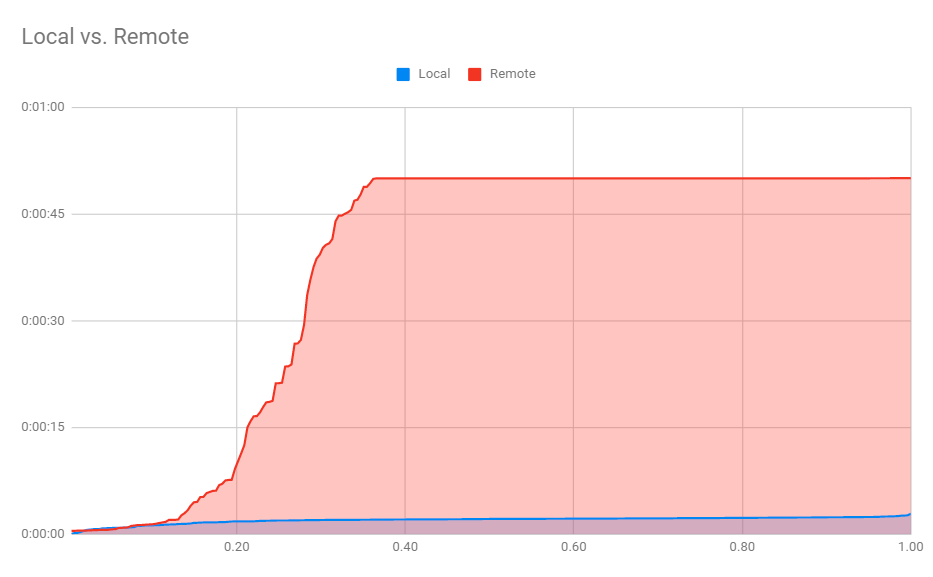
\includegraphics[width=\linewidth]{imagenes/queryRuntimeCompared.png}
        \caption{Comparison of local and remote query times}
        \label{fig:runtimeCompare}
\end{figure}

In our local query times, all queries run in under 3 seconds, with around 8\% running in under 1 second, and 25\% running in under 2 seconds.

\begin{figure}[h]
    \centering
        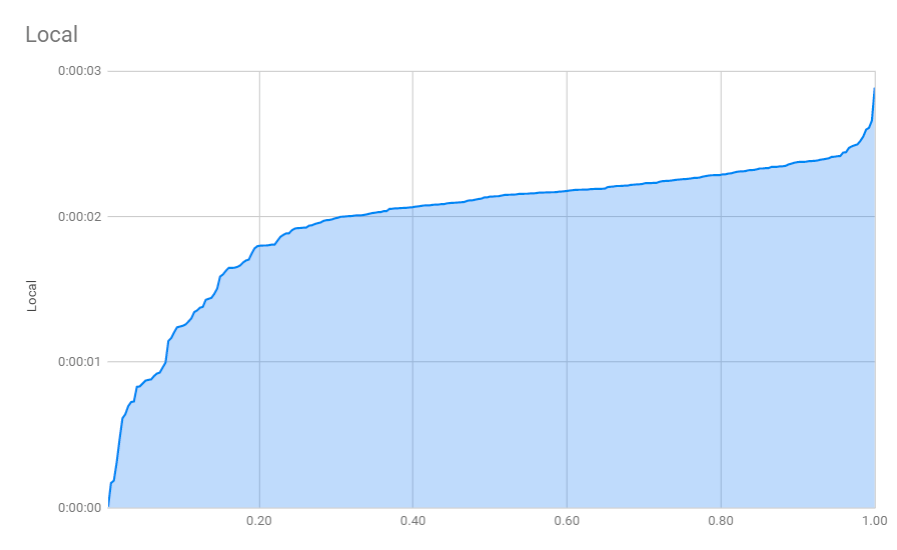
\includegraphics[width=\linewidth]{imagenes/localQueryRuntime.png}
        \caption{Local query times}
        \label{fig:runtimeLocal}
\end{figure}

\subsection{Results approximations}

In our previous section we presented the query runtimes for our 268 queries. In this section we present the results of those queries: How similar are the values that our system suggests compared against the exact values from the remote endpoint? It is worth mentioning that we can only compare  results for the 78 queries that did return values from the remote endpoint. 

For this, we expect to get an over-approximation of our suggested values, meaning that we return all of the exact values and some incorrect values as well. 

\begin{figure}[ht]
    \centering
        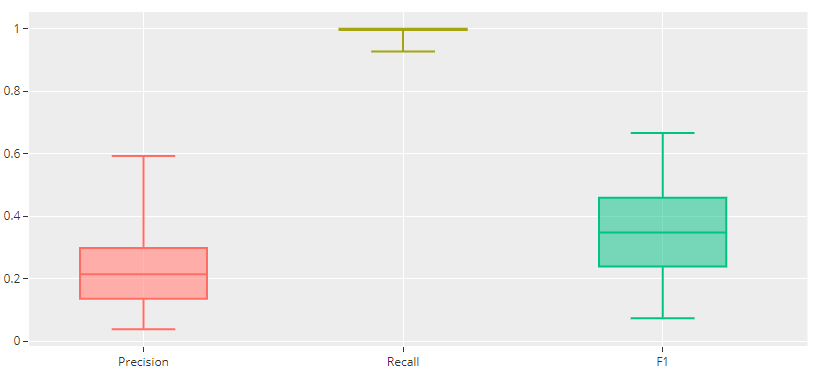
\includegraphics[width=\linewidth]{imagenes/resultsCandleStick.png}
        \caption{Precision, Recall, F1}
        \label{fig:resultsCandles}
\end{figure}

In \autoref{fig:resultsCandles} we present the minimum and maximum results for precision, recall and F1. At the start of this chapter we mentioned that we expected a high value of recall, given that we should suggest all true-positives and that we should not have false-negatives inside our suggestions. The results in this sense are very similar to what we expected: Our results have an average of 99.40\% of recall, where the slight drop in recall is due to changes in the data between our indexing process and querying the live endpoint. Regarding precision: since we are providing over-approximated suggestions, our precision is expected to be low. As an average, we have 22\% precision and 35\% F1.

It is important to note that the results that we can provide are based on the dataset dump, where any changes on the remote endpoint database will not be reflected in our local index. This implies that for any changes in the remote database, our measures will deteriorate in time against the live ones.

% ##############################################################################################
% ##############################################################################################
% ##############################################################################################

\section{Discussion}

We started this chapter by raising some questions about our system performance. In regards to the required time for indexing the Wikidata dump, from our results we can see that indexing is a time consuming process that can take up to 109 hours to run. Considering that a new dump is generated every week or every two weeks, our system could be scheduled to run after one of the dump generation tasks.

We also considered the space requirements involved for our backend. The system requirements regarding disk space allow our system to keep a version running; sorting our index files requires a peak physical disk space of 300GB, which is not too demanding for modern hardware.

Comparing our result times and correctness against SPARQL, our system can deliver results within 3 seconds with 25\% precision on average versus exact results. While interactive user suggestions usually can be expected within the milliseconds range, we consider that our 3 second suggestions are acceptable while using the system, especially if compared against the timeouts that most of the tested queries encounter when computed on the remote SPARQL endpoint.

Related to correctness, since our specialized index is built from a dump, which is generated every week, the correctness of the suggestions will gradually reduce: some triples which establish  domain and range relations might be removed or new ones might be added in the online dataset, which in turn generates a difference between our results and the SPARQL endpoint results. This might be avoided by periodically generating a new specialized index, or implementing a delta mechanism to keep the system up to date. This however is out of our current scope.
